\chapter{Redes Neuronales y Modelos Generativos}\label{chap:redes-neuronales-y-modelos-generativos}  % MARK: Redes Neuronales y Modelos Generativos
Este capítulo introduce los modelos generativos, empezando por las redes neuronales, viendo las versiones más simples, y terminando con sus variantes basadas en la distancia de Wasserstein. Para ello, se empieza por definir lo que es una red neuronal.

\RED[inline]{¿Se podría poner en esta parte la razón por la que estoy incluyendo a las redes neuronales? ¿O explicar la forma en que estará estructurado el capítulo? (breve intro redes neuronales, GANs, WGANs, AE, WAE y por último la aplicación con baricentros de Wasserstein).}

\section{Redes Neuronales}\label{sec:redes-Neuronales}  % MARK: Redes Neuronales
En el último tiempo se ha visto un auge en el uso de las redes neuronales en diversas áreas de la ciencia y la tecnología. Esto se debe a que las redes neuronales han demostrado ser muy efectivas en la resolución de problemas complejos, como la clasificación de imágenes, el procesamiento de lenguaje natural, y la generación de texto e imágenes, entre otros.

Este capítulo introduce los conceptos básicos de las redes neuronales, aunque no se profundiza en los detalles de su funcionamiento. Para ello, se recomienda al lector revisar la literatura especializada en el tema, tales como ``Deep learning'' \cite{goodfellow2016deep} y ``Deep learning architectures'' \cite{calin2020deep}.\RED{Estos nombres en inglés deberían estar en cursiva? O los nombres de los libros, en sí, deberían de estar en cursiva?}

El proceso de definición de una red neuronal comienza estableciendo algunas constantes preliminares. El origen de los nombres de las siguientes definiciones se entienden con el Ejemplo~\ref{ex:ejemplo-red-neuronal}. Se define por $L\in\N$ la \emph{profundidad} de la red, la cuál determina el número de \textit{capas ocultas} y la \textit{capa de salida} que tiene la red. Para $\ell \in \left\{ 0,\ldots, L \right\}$, se define $d_\ell\in\N$ como el \emph{número de neuronas de la capa $\ell$}.

De esta manera, una red neuronal prealimentada (FFNN por sus siglas en inglés: \textit{feed-forward neural net}) es simplemente una composición de funciones lineales y no lineales. Más precisamente, para $L$ funciones lineales $\{ g^{(\ell)}_{\vth_\ell} \colon \R^{d_{\ell-1}} \to \R^{d_{\ell}} \mid \ell = 1, \ldots, L \}$, definidas por
\begin{align*}
	g^{(\ell)}_{\vth_\ell} \colon \R^{d_{\ell-1}} & \to \R^{d_\ell}                                                        \\
	\vx_\ell                                      & \mapsto g^{(\ell)}_{\vth_\ell}(\vx_\ell) = \vW_\ell \vx_\ell + b_\ell,
\end{align*}
donde $\vth_\ell = (\vW_\ell, b_\ell)$ corresponden a los \textit{parámetros}, $\vW_\ell \in \R^{d_{\ell} \times d_{\ell-1}}$ a los \emph{pesos} y $b_\ell \in \R^{d_\ell}$ al \emph{sesgo}\footnote{En español también se suele referir al sesgo por su anglicismo: \textit{bias}.} de la capa $\ell$.
Se considera además $L$ funciones no lineales $\{ \sigma^{(\ell)} \colon \R \to \R \mid \ell = 1, \ldots, L \}$, a las cuales llamaremos \emph{funciones de activación}. Por convención, se asume que las funciones de activación son aplicadas elemento a elemento, es decir, que si $\sigma$ es una función de activación, entonces $\sigma(\vx) = \left( \sigma(x_1), \ldots, \sigma(x_n) \right)$ para $\vx = (x_1, \ldots, x_n) \in \R^n$.

Estas funciones lineales y no lineales se pueden componer para formar una red neuronal:
\begin{equation}
	f_{\vth}(\vx) = \sigma^{(L)} \circ g^{(L)}_{\vth_L} \circ \sigma^{(L-1)} \circ g^{(L-1)}_{\vth_{L-1}} \circ \cdots \circ \sigma^{(1)} \circ g^{(1)}_{\vth_{1}}(\vx).
\end{equation}
A este tipo de modelos se les suele representar como grafos dirigidos acíclicos, describiendo cómo las funciones se encuentran compuestas entre sí.

\begin{remark}
	Cabe destacar que es necesario que las funciones de activación $\sigma$ sean no lineales. Pues si lo fueran, entonces la red sería una composición de funciones lineales, lo que resulta en una única función lineal. La problemática que se tendría con esta definición es que no habría ninguna ganancia con hacer la red más profunda, pues todo colapsaría a una única capa. Es por este motivo que a estas funciones se les llama \textbf{funciones de activación}, pues ``activan'' la no-linealidad de la red, permitiendo que esta pueda aprender funciones más complejas.
\end{remark}


\begin{example}\label{ex:ejemplo-red-neuronal}
	En la Figura~\ref{fig:ejemplo-red-neuronal} se puede observar una representación de una red neuronal con tres capas ocultas y una capa de salida.

	\begin{figure}[htbp]
		\centering
		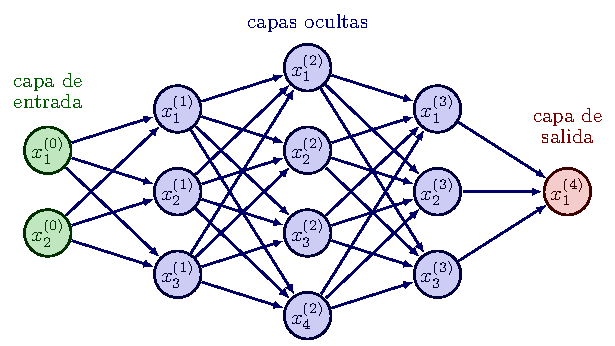
\includegraphics[width=0.5\textwidth]{img/neural_network/neural_network_feed_forward.pdf}
		\caption{Representación de una FFNN con cuatro capas. Elaboración propia.}
		\label{fig:ejemplo-red-neuronal}
	\end{figure}

	En este caso, la red neuronal se encuentra compuesta por cinco capas: una de entrada con $d_0 = 2$, tres ocultas con $d_1 = 3$, $d_2 = 4$, $d_3 = 3$, y una de salida con $d_4 = 1$. Cada uno de los nodos $x_i^{(\ell)}$ corresponde a la $i$-ésima \textit{neurona} de la capa $\ell$. Es este el motivo de porqué a $d_\ell$ se les refiere como el número de neuronas de la capa $\ell$. Además, se puede notar que, sin contar la capa de entrada, la red neural tiene una profundidad de $L = 4$ capas, de ahí que se le llame profundidad de la red.

	En este caso, la función $g^{(\ell)}_{\vth_\ell}$ es representada a través de los arcos que conectan las neuronas de la capa $\ell-1$ con las neuronas de la capa $\ell$. Por otro lado, las funciones de activación $\sigma^{(\ell)}$ se encuentran implícitamente utilizadas al definir recursivamente los vectores de neuronas $x^{(\ell)} \in \R^{d_\ell}$ de la siguiente manera:
	\begin{equation}
		x^{(\ell)} =
		\begin{cases}
			\vx,                                                         & \text{si } \ell = 0,           \\
			\sigma^{(\ell)} \circ g^{(\ell)}_{\vth_\ell} (x^{(\ell-1)}), & \text{en cualquier otro caso.}
		\end{cases}
		\quad \forall \ell = 0, \ldots, L.
	\end{equation}
	Es evidente concluir que la salida de la red neuronal es $f_{\vth}(\vx) = x^{(L)}$.
\end{example}

La razón por la que las redes neuronales han tenido tanto éxito en los últimos años se debe a que estas son capaces de aprender funciones muy complejas, siempre y cuando estas posean el número de parámetros suficientes y la cantidad de datos necesario.
Este hecho es demostrado por George Cybenko en 1989 en su Teorema de Aproximación Universal (UAT por sus siglas en inglés) \cite{cybenko1989approximation}.

A pesar de que la primera versión del UAT fue propuesta por Cybenko en 1989, el teorema fue popularizado por Kurt Hornik en 1991 \cite{hornik1991approximation}, debido a que en el teorema de Cybenko utiliza una función de activación sigmoide, mientras que en la versión de Hornik lo extiende a una función de activación continua. Por este motivo, es que a continuación se presenta la versión de Hornik del UAT.
\begin{theorem}[Teorema de Aproximación Universal \cite{hornik1991approximation}]\label{thm:universal-approximation-theorem}
	Sea $\sigma \in \ContSpace[\R, \R]$ una función de activación continua.
	Sean $d_0, d_2 \in \N$, números naturales, $K \subseteq \R^{d_0}$ un conjunto compacto y $f \in \ContSpace[K, \R^{d_2}]$ la función a aproximar.
	Entonces, $\sigma$ no es polinomial sí y sólo sí para cada $\epsilon > 0$, existe $d_1\in\N$, $\vW \in \R^{d_1 \times d_0}$, $b \in \R^{d_1}$ y $C \in \R^{d_2 \times d_1}$ tal que:
	\begin{equation}
		\sup_{\vx \in K} \left\| f(\vx) - C \cdot \sigma(\vW \cdot \vx + b) \right\| < \epsilon.
	\end{equation}
\end{theorem}

\begin{remark}
	El Teorema~\ref{thm:universal-approximation-theorem} establece que una red neuronal de una única capa oculta con una función de activación no polinomial (como por ejemplo, una sigmoide) es capaz de aproximar cualquier función continua en un conjunto compacto $K$ con un error arbitrariamente pequeño. Sin embargo, este teorema no establece cuántas neuronas en la capa oculta son necesarias para aproximar dicha función, ni tampoco establece cómo se deben de escoger los parámetros de la red neuronal.
\end{remark}

Con el paso de los años, se han propuesto diversas versiones del UAT. Sin embargo, el Teorema~\ref{thm:universal-approximation-theorem} ya ilustra de manera efectiva por qué las redes neuronales son tan efectivas en la aproximación de funciones.

Este capítulo concluye destacando la existencia de múltiples variantes de las redes neuronales, entre las que se incluyen las Redes Neuronales Convolucionales (CNN por sus siglas en inglés) y las Redes Neuronales Recurrentes (RNN por sus siglas en inglés). Estas variantes han ganado popularidad en los campos de la visión computacional y del procesamiento de lenguaje natural, respectivamente. Específicamente, en el presente trabajo se emplean las Redes Neuronales Convolucionales.



\section{Redes Generativas Adversarias}\label{sec:redes-generativas-adversarias-GAN}  % MARK: Redes Generativas Adversarias

Comencemos esta sección imaginando la siguiente situación\footnote{Este ejemplo es una adaptación y fue inspirado de \cite[min. 4:32]{santana2017creando}}:
\begin{quotation}
	\textit{Supongamos que hay un ladrón que desea engañar a un policía entregándole un billete falso. El ladrón, que es un inexperto, le entrega una servilleta, con una cara dibujada en ella, y que en el otro lado de la servilleta tiene escrito: ``\emph{esto vale un millón de dólares}''. El policía, que ha sido entrenado en la detección de billetes falsos, revisa el billete para comprobar que, efectivamente, es un billete falso.}

	\textit{Sin embargo, en vez de enviar a la cárcel al ladrón, lo que hace es decirle al ladrón cuales fueron sus fallos, y de qué manera puede este mejorar en sus falsificaciones. Por su parte, el policía también se entrena más y más en la detección de billetes falsos, pues puede que en algún momento, el ladrón se vuelva tan bueno en la elaboración de billetes falsos, que llegue a engañar al policía con uno de sus billetes.}
\end{quotation}

\begin{figure}[htbp]
	\centering
	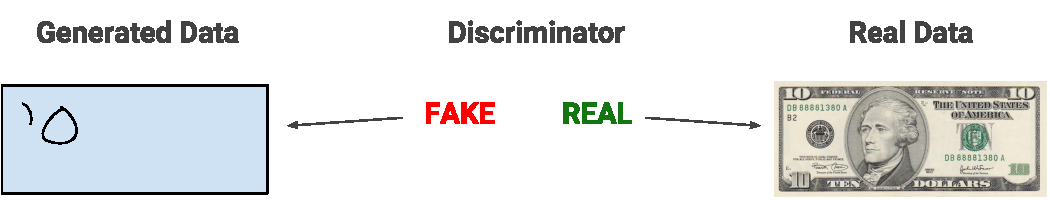
\includegraphics[width=0.7\textwidth]{img/gan/bad_gan.pdf}\vspace{0.6cm}
	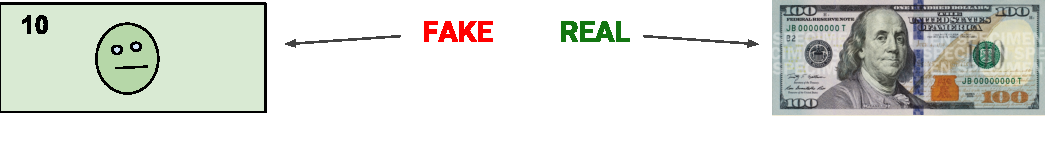
\includegraphics[width=0.7\textwidth]{img/gan/ok_gan.pdf}
	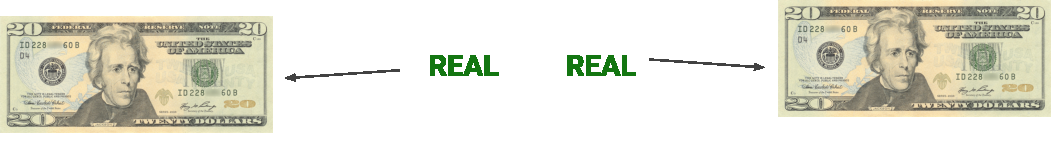
\includegraphics[width=0.7\textwidth]{img/gan/good_gan.pdf}
	\caption{Visualización gráfica de la analogía del ladrón y el policía en las GAN. Imagen obtenida de \cite{googlegan}.}
	\label{fig:gan-analogy}
\end{figure}

El marco de las Redes Generativas Adversarias (GAN), introducido en el trabajo de Goodfellow et al. \cite{goodfellow2014generative}, es en esencia, la analogía del ladrón y el policía.
La GAN define un juego donde el objetivo de la \emph{generadora} (el ladrón) es la de generar muestras que parezcan reales, mientras que el objetivo de la \emph{discriminadora} (el policía) es el de clasificar las muestras como verdaderas o falsas.
En este caso, la generadora se entrena para engañar a la discriminadora, y la discriminadora se entrena para detectar la falsedad de las muestras generadas.

En la siguiente subsección define formalmente una GAN, presenta los teoremas de convergencia de la GAN, y se describe el algoritmo de entrenamiento de una GAN. En las subsecciones posteriores a esta se presentan las variantes de las GAN, como las WGAN, WGAN-GP y WGAN-LP, elementos necesarios para una de las partes de esta tesis.

\subsection{GAN}\label{ssec:GAN}
% MARK: GAN

En este trabajo de tesis se plantea una definición formal de una GAN, en el contexto no paramétrico, y utilizando medidas de probabilidades generales. Este enfoque es diferente al que se plantea en el \textit{paper} original \cite{goodfellow2014generative}, donde se utiliza una formulación no paramétrica, pero asumiendo que las medidas de probabilidad poseen densidad. Por tanto, se utiliza la formulación presentada en \cite{wikipediagan}, la cuál se basa en medidas de probabilidad generales, aunque se reescriben los teoremas y demostraciones para garantizar su formalidad. Estos se pueden encontrar en el Anexo~\ref{chap:demostraciones-adicionales-teos-gan}.

Desde el punto de vista de la teoría de juegos, la GAN se define como un juego de dos jugadores: una \textit{generadora} $\Prob_G$, donde su conjunto de estrategias es $\ProbSpace[\cX]$ (con $\cX$ el \textit{conjunto de referencia}, e.g. $\cX=[0, 1]^{n_1\times n_2}$ para un conjunto de imágenes), y una \textit{discriminadora} $\Prob_D(\dd y \mid x)$, donde su conjunto de estrategias es el conjunto de kernels Markovianos. Con esto, la GAN es un juego de suma cero con la siguiente función valor objetivo:
\begin{equation}
	\label{eq:gan-objective}
	V(\Prob_G, \Prob_D)
	= \Exp_{X\sim\Prob_G}{\Exp_{Y \sim \Prob_D(\dd y \mid X)} \left[ \ln Y \right]}
	+ \Exp_{\tilde X\sim\Prob_G}{\Exp_{Y \sim \Prob_D(\dd y \mid \tilde X)} \left[ \ln (1 - Y) \right]},
\end{equation}
donde la generadora busca minimizar la función valor, mientras que la discriminadora busca maximizar esta cantidad.

El objetivo final de la generadora es el de encontrar una distribución $\Prob_G$ tal que se aproxime a una distribución de referencia $\Prob_X \in \ProbSpace[\cX]$ (del cuál se tiene acceso a través de una medida empírica $\hat \Prob_X = \frac{1}{N} \sum_{i=1}^{N} \delta_{x_i}$). Por el otro lado, el objetivo de la discriminadora es el de clasificar las muestras verdaderas y falsas, asignándole valores cercano a 1 y 0 respectivamente.

El siguiente teorema nos habla acerca de la naturaleza del discriminador óptimo:

\begin{theorem}[El discriminador óptimo calcula la divergencia de JS]
	\label{thm:gan-optimal-discriminator}
	Para cualquier estrategia de generador $\Prob_G$ fijo, existe un único discriminador óptimo $\Prob_D^\ast$ que maximiza la función objetivo \eqref{eq:gan-objective}, el cuál toma una forma determinista por medio de $\Prob_D^\ast(\dd y \mid x) = \delta_{D^\ast(x)}(\dd y)$, donde $D^\ast(x) = \dv{\Prob_X}{(\Prob_G+\Prob_X)}$. En tal caso, la función valor toma la siguiente forma:
	\begin{equation}
		V(\Prob_G, \Prob_D^\ast) = \JS{\Prob_X}{\Prob_G} - 2 \ln 2.
	\end{equation}
\end{theorem}

\begin{proof}
	La demostración de este teorema se encuentra en el Anexo~\ref{chap:demostraciones-adicionales-teos-gan}.
\end{proof}

Este teorema nos dice que el discriminador óptimo es aquel que calcula la divergencia de Jensen-Shannon entre la distribución de referencia $\Prob_X$ y la distribución generada $\Prob_G$, salvo una constante. Además, nos dice que el discriminador toma una forma determinista, de forma que bastaría con buscar una función (como por ejemplo, una red neuronal) $D\colon\cX\to [0, 1]$ tal que la aproxime.

Dado que para cada generador $\Prob_G$ existe un único discriminador óptimo $\Prob_D^\ast$, entonces tiene sentido definir la siguiente función:
\begin{equation}
	C(\Prob_G) \eqdef V(\Prob_G, \Prob_D^\ast) = \JS{\Prob_X}{\Prob_G} - 2 \ln 2.
\end{equation}
El siguiente teorema nos dice que existe un único generador óptimo $\Prob_G^\ast$ que minimiza la función $C(\Prob_G)$, y que este corresponde a la distribución de referencia $\Prob_X$:

\begin{theorem}\label{thm:gan-optimal-generator}
	El mínimo global de la función $C(\Prob_G)$ se alcanza en $\Prob_G^\ast = \Prob_X$, y el valor mínimo es $C(\Prob_X) = - \ln 4$.
\end{theorem}

\begin{proof}
	La demostración de este teorema se encuentra en el Anexo~\ref{chap:demostraciones-adicionales-teos-gan}.
\end{proof}

En la práctica, la forma de implementar la generadora es a través de un \emph{modelo generativo de espacio latente}. Esto es,
\begin{equation}\label{eq:generative-model}
	\Prob_G (\dd x) \eqdef \int_\cZ \Prob_G(\dd x \mid z) \; \Prob_Z \left( \dd z\right),
\end{equation}
donde $\cZ$ es el espacio de las variables latentes, y $\Prob_Z \in \ProbSpace[\cZ] $ es la distribución del espacio latente (típicamente se utiliza la distribución Gaussiana o Uniforme).

Por simplicidad, el modelo generativo $\Prob_G (\dd x \mid z)$ se mapea de forma determinista a través de $\Prob_G (\dd x \mid z) = \delta_{G(z)}(\dd x)$, utilizando una función $G\colon \cZ \to \cX$, la cuál se estima a través de una red neuronal $G_\theta$. Por otro lado, el Teorema~\ref{thm:gan-optimal-discriminator} dice que, en el óptimo, el discriminador toma una forma determinista, de forma que basta con buscar una función $D\colon\cX\to [0, 1]$, la cual también se estima a través de una red neuronal $D_\varphi$.

\FM{Agregar una explicación de las funciones de pérdida para este caso, explicar qué cosas buscan minimizar/maximizar y describir el algoritmo de entrenamiento.}

Con el fin de definir un algoritmo para entrenar una GAN, se definen las siguientes funciones de pérdida para la generadora y la discriminadora:
\begin{align}
	\cL_{\mathrm{disc}} & = -\frac{1}{N}\sum_{i=1}^{N} \Big[ \ln D_\varphi(x_i) + \ln \qty\big(1 - D_\varphi(G_\theta(z_i))) \Big], \\
	\cL_{\mathrm{gen}}  & = - \frac{1}{N}\sum_{i=1}^{N} \ln \qty\big(D_\varphi(G_\theta(z_i))),
\end{align}
donde $\{x_i\}_{i=1}^{N} \sim \Prob_X$ y $\{z_i\}_{i=1}^{N} \sim \Prob_Z$ son muestras del conjunto de entrenamiento y del espacio latente, respectivamente. La función de pérdida $\cL_{\mathrm{disc}}$ proviene de buscar maximizar la función objetivo \eqref{eq:gan-objective}, mientras que la función de pérdida $\cL_{\mathrm{gen}}$ se deriva de buscar minimizar la misma función objetivo.

De esta manera, el Algoritmo~\ref*{alg:GAN} describe la forma de estimar los parámetros $\theta$ y $\varphi$ de la generadora y la discriminadora, respectivamente. Usualmente, el flujo de este algoritmo se realiza en dos pasos: primero se actualiza la discriminadora $D_\varphi$ por $N_d$ iteraciones, y luego se actualiza la generadora $G_\theta$ por una iteración. Este proceso se repite hasta que los parámetros $\theta$ converjan.

\begin{algorithm}[H]
	\caption{Entrenamiento de una Red Generativa Adversaria}\label{alg:GAN}
	\begin{algorithmic}[1]
		\Require Tamaño del batch $N$ y número de iteraciones para el discriminador $N_d$.
		\State Inicializar los parámetros de la generadora $G_\theta$ y la discriminadora $D_\varphi$.
		\While{$\theta$ no ha convergido}
		\For{$t=1,\ldots,N_d$}
		\State Muestrear $\{x_i\}_{i=1}^{N} \sim \Prob_X$ desde el conjunto de entrenamiento.
		\State Muestrear $\{z_i\}_{i=1}^{N} \sim \Prob_Z$ desde el espacio latente.
		\State $\cL_{\mathrm{disc}} \gets -\frac{1}{N}\sum_{i=1}^{N} \Big[ \ln D_\varphi(x_i) + \ln \qty\big(1 - D_\varphi(G_\theta(z_i))) \Big]$
		\State Actualizar $D_\varphi$ por medio de descenso de gradiente en $\pdv{\varphi} \cL_{\mathrm{disc}}$.
		\EndFor
		\State Muestrear $\{z_i\}_{i=1}^{N} \sim \Prob_Z$ desde el espacio latente.
		\State $\cL_{\mathrm{gen}} \gets - \frac{1}{N}\sum_{i=1}^{N} \ln \qty\big(D_\varphi(G_\theta(z_i)))$
		\State Actualizar $G_\theta$ por medio de descenso de gradiente en $\pdv{\theta} \cL_{\mathrm{gen}}$.
		\EndWhile
	\end{algorithmic}
\end{algorithm}

\begin{remark}
	El Algoritmo~\ref{alg:GAN} empieza por determinar el óptimo de $\max_D V( \Prob_G , \Prob_D )$, el cuál proporciona una aproximación para la divergencia de Jensen-Shannon entre $\Prob_X$ y $\Prob_G$. Luego, actualiza la generadora $G$ para minimizar dicha divergencia. Con este procedimiento, la distribución $\Prob_G$ converge a la distribución de referencia $\Prob_X$ \textbf{utilizando la divergencia de Jensen-Shannon}.
\end{remark}

Es común que las arquitecturas de tipo GAN sean representadas como en la Figura~\ref{fig:gan-diagram}. En esta figura, se puede observar que la generadora $G$ toma una variable latente $z$ y la mapea a una muestra $\tilde x$, mientras que la discriminadora $D$ toma una muestra $x$ y la clasifica como verdadera o falsa.

\begin{figure}[H]
	\centering
	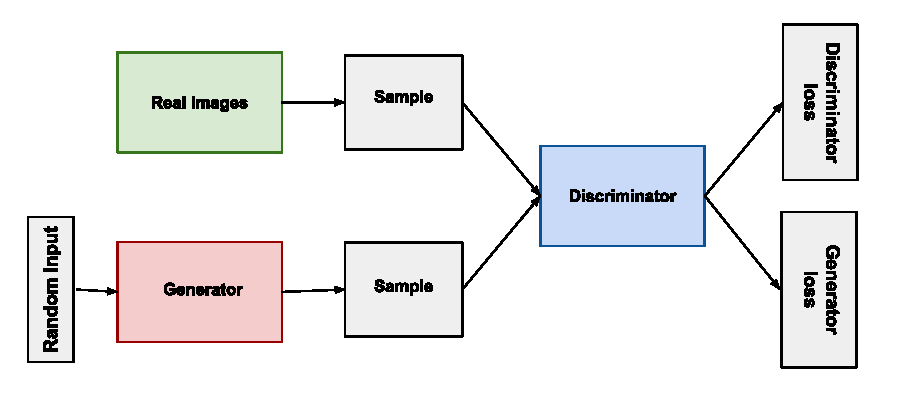
\includegraphics[width=0.75\textwidth]{img/gan/gan_diagram.pdf}
	\caption{Representación gráfica de la arquitectura de una GAN. Imagen obtenida de \cite{googlegan}.}
	\label{fig:gan-diagram}
\end{figure}


\FM[inline]{Si es que en el futuro se puede, modificar esta figura para que coincida más con la descripción}

% Teorema de la GAN: Convergencia en divergencia Jensen-Shannon

% Ejemplos?


\subsection{Wasserstein GAN}\label{ssec:wasserstein-gan}  % MARK: WGAN

La Wasserstein GAN (WGAN) \cite{arjovsky2017wasserstein} es una variante de las GANs que propone una nueva función de pérdida basada en la distancia de Wasserstein, en lugar de la divergencia de Jensen-Shannon. La principal ventaja de la WGAN es que es más estable y efectiva en la generación de datos, evitando problemas como el modo de colapso y el desvanecimiento del gradiente.

La función de pérdida se basa en el teorema de dualidad de Kantorovich-Rubinstein, el cuál se enuncia a continuación:
\begin{theorem}[Teorema de dualidad de Kantorovich-Rubinstein \cite{villani2009optimal}]\label{thm:dualidad-kantorovich-rubinstein}
	Sean $\Prob, \ProbQ \in \WassersteinSpace[1]{\cX}$ dos medidas de probabilidad en un espacio métrico $\cX$. Entonces, la distancia de Wasserstein entre $\Prob$ y $\ProbQ$ se puede expresar como:
	\begin{equation}\label{eq:dualidad-kantorovich-rubinstein}
		\Wasserstein[1]{\Prob}{\ProbQ} = \sup_{f \in \Lip[\cX]} \left\{ \Exp_{X\sim \Prob} [f(X)] - \Exp_{\tilde X \sim \ProbQ} [f(\tilde X)] \right\}.
	\end{equation}
\end{theorem}

Inspirados en este teorema, los autores de la WGAN \cite{arjovsky2017wasserstein} reemplazan el anterior juego de la GAN por el siguiente:
\begin{equation}\label{eq:wgan-game}
	(P_{\mathrm{WGAN}}) \quad \min_{G} \max_{f \in \Lip[\cX]} \Exp_{X\sim \Prob_X} [f(X)] - \Exp_{\tilde X \sim \Prob_G} [f(\tilde X)],
\end{equation}
donde la función $G$ es la \textit{generadora} y $f$ es la \textit{función crítica}. Se puede destacar que en este juego, el primer objetivo es obtener una estimación de la distancia de Wasserstein, para después utilizar esta estimación para minimizar la distancia entre la distribución real y la generada.

En la práctica, se utilizan las redes neuronales $G_\theta: \cZ \to \cX$ y $f_\omega: \cX \to \R$ para aproximar la generadora y la función crítica, respectivamente.
La generadora $G_\theta$ busca, como en el caso de la GAN, minimizar la distancia entre la distribución real y la generada, mientras que la función crítica $f_\omega$ busca maximizar la expresión en~\eqref{eq:dualidad-kantorovich-rubinstein}, con la restricción de que sea $1$-Lipschitz.

Este procedimiento define a la función de pérdida como
la diferencia entre la media de la función crítica evaluada en las muestras reales y generadas, lo que proporciona una estimación de la distancia de Wasserstein:
\begin{equation}\label{eq:wasserstein-estimation}
	\widehat W_N^{(1)} (
	\omega, \theta, x, z
	)
	\eqdef \frac{1}{N}\sum_{i=1}^{N} f_\omega(x_i) - \frac{1}{N}\sum_{i=1}^{N} f_\omega(G_\theta(z_i)),
\end{equation}
donde $x = (x_i)_{i=1}^{N} \sim \Prob_X$ y $z = (z_i)_{i=1}^{N} \sim \Prob_Z$ son muestras de las distribuciones reales y del espacio latente, respectivamente.

Más específicamente, las funciones de pérdida para la generadora y la función crítica son las siguientes:
\begin{align}
	\cL_{\mathrm{critic}}(\omega)
	 & = -\widehat W_N^{(1)} (
	\omega, \theta, x, z
	)
	= \frac{1}{N}\sum_{i=1}^{N} f_\omega(G_\theta(z_i)) - \frac{1}{N}\sum_{i=1}^{N} f_\omega(x_i),
	\\ \cL_{\mathrm{gen}}(\theta)
	 & = \widehat W_N^{(1)} (
	\omega, \theta, x, z
	)
	= -\frac{1}{N}\sum_{i=1}^{N} f_\omega(G_\theta(z_i)).
\end{align}
Destacando que, como la función de pérdida busca maximizar $\cL$, entonces este cambia su signo. Por otro lado, la función de pérdida de la generadora busca minimizar $\cL$, pero descarta los términos que no dependan de $\theta$.

Con el fin de asegurarse que la función crítica $f_\omega$ sea $1$-Lipschitz, en el trabajo original se proponía la restricción de que los pesos de la red fueran acotados. Esta restricción empeora el desempeño de la red, por lo que se han propuesto otras alternativas para garantizar que la red neuronal $f_\omega$ sea $1$-Lipschitz. Estas variaciones se revisarán en las siguientes subsecciones.

Paso seguido, la generadora utiliza la aproximación de la distancia de Wasserstein para minimizar la distancia entre la distribución real y la generada (recordando que esta se obtiene a través de un modelo generativo de espacio latente).

De este modo, el algoritmo de entrenamiento de la WGAN se resume en el Algoritmo~\ref{alg:WGAN}.

\begin{algorithm}[H]
	\caption{Entrenamiento de una Wasserstein GAN}\label{alg:WGAN}
	\begin{algorithmic}[1]
		\Require Tamaño del batch $N$, número de iteraciones para el discriminador $N_d$ y el parámetro de clipping $c$.
		\State Inicializar los parámetros de la generadora $G_\theta$ y la función crítica $f_\omega$.
		\While{$\theta$ no ha convergido}
		\For{$t=1,\ldots,N_d$}
		\State Muestrear $\{x_i\}_{i=1}^{N} \sim \Prob_X$ desde el conjunto de entrenamiento.
		\State Muestrear $\{z_i\}_{i=1}^{N} \sim \Prob_Z$ desde el espacio latente.
		\State $\cL_{\mathrm{critic}} \gets
			\frac{1}{N} \sum_{i=1}^{N} f_{\omega}(G_\theta(z_i)) - \frac{1}{N} \sum_{i=1}^{N} f_{\omega}(x_i)$ \Comment{$\cL_{\mathrm{critic}} = -\widehat W_N^{(1)}$}
		\State Actualizar $f_{\omega}$ por medio de descenso de gradiente en $\pdv{\omega} \cL_{\mathrm{critic}}$.
		\State $\omega \gets \text{clip}(\omega, -c, c)$
		\EndFor
		\State Muestrear $\{z_i\}_{i=1}^{N} \sim \Prob_Z$ desde el espacio latente.
		\State $\cL_{\mathrm{gen}} \gets - \frac{1}{N}\sum_{i=1}^{N} f_\omega(G_\theta(z_i))$ \Comment{
		$\cL_{\mathrm{gen}} = \widehat W_N^{(1)}$
		}
		\State Actualizar $G_\theta$ por medio de descenso de gradiente en $\pdv{\theta} \cL_{\mathrm{gen}}$.
		\EndWhile
	\end{algorithmic}
\end{algorithm}

\FM[inline]{Agregar la explicación de que ahora, gracias a que se utiliza la distancia de wasserstein, estas medidas terminan convergiendo débilmente a la distribución de referencia (lo que lo hace más fácil de converjer)}

\subsection{Wasserstein GAN con Gradiente Penalizado}\label{ssec:}  % MARK: Wasserstein GAN con Gradiente Penalizado
Los autores de la WGAN reconocen que la restricción de que los pesos de la red sean acotados no es la mejor forma de garantizar que la función crítica sea $1$-Lipschitz. Por ello, proponen una nueva forma de garantizar esta restricción, mediante la penalización de gradientes \cite{gulrajani2017improved}. Esta técnica es llamada Wasserstein GAN con Gradiente Penalizado (WGAN-GP).

La idea por detrás de esta técnica proviene del siguiente corolario:

\begin{corollary}[Corolario 1 de \cite{gulrajani2017improved}]\label{cor:gradiente-penalizado}
	Sea $f^\ast$ la función que minimiza el problema de optimización del Teorema de dualidad de Kantorovich-Rubinstein (ver la Ecuación~\eqref{eq:dualidad-kantorovich-rubinstein} del Teorema~\ref{thm:dualidad-kantorovich-rubinstein}). Entonces, la norma del gradiente de $f^\ast$ es $1$ en casi todo punto bajo las distribuciones $\Prob$ y $\ProbQ$. Es decir,
	\begin{equation}
		\Exp_{Y\sim\tau} \qty\Big[ \norm{\nabla f^\ast(Y)} ] = 1,
	\end{equation}
	donde $\tau$ es una distribución definida de forma que $u\sim\Uniform[0, 1]$, y $Y = uX + (1-u)\tilde X$ con $X\sim\Prob$ y $\tilde X\sim\ProbQ$.
\end{corollary}

La idea que hay por detrás de este corolario, es que basta penalizar la función de pérdida de la función crítica $f_\omega$ cuando su gradiente no sea $1$, para garantizar que esta sea $1$-Lipschitz. Es decir, que intercambian el problema de optimización de~\eqref{eq:wgan-game} por el siguiente:
\begin{equation}
	(P_{\mathrm{WGAN-GP}}) \quad \min_{G} \max_{f} \Exp_{X\sim \Prob_X} [f(X)] - \Exp_{\tilde X \sim \Prob_G} [f(\tilde X)] + \lambda \Exp_{Y\sim\tau} \qty\Big[ \qty(\norm{\nabla f(Y)} - 1)^2 ],
\end{equation}
donde $\lambda$ es un coeficiente de penalización y $\tau$ es una distribución definida como en el Corolario~\ref{cor:gradiente-penalizado}.

Además, como este es una penalización para la función crítica, entonces la función de pérdida de la generadora se mantiene igual a la de la WGAN. De esta forma, la función de pérdida para la función crítica se define de la siguiente manera:
\begin{align}
	p(\omega, x, \tilde x) & \eqdef \frac{1}{N} \sum_{i=1}^{N} \qty(
	\norm{\nabla f_\omega(u_i x_i + (1-u_i) \tilde x_i)} - 1
	)^2 ,
	\\ \cL_{\mathrm{critic}}(\omega) & \eqdef
	\frac{1}{N} \sum_{i=1}^{N} f_\omega(x_i) - \frac{1}{N} \sum_{i=1}^{N} f_\omega(\tilde x_i)
	+ \lambda p(\omega),
\end{align}
donde $u = (u_i)_{i=1}^{N} \sim \Uniform[0, 1]$, $x = (x_i)_{i=1}^{N} \sim \Prob_X$ y $\tilde x = (\tilde x_i)_{i=1}^{N} \sim \Prob_G$ son muestras de las distribuciones reales y generadas, respectivamente.


\begin{algorithm}[H]
	\caption{Penalización del Gradiente}\label{alg:gradient-penalty}
	\begin{algorithmic}[1]
		\Function{gradPenalty}{$\omega$, $x$, $\tilde x$}
		\State Muestrear $u = (u_i)_{i=1}^N \sim \Uniform[0, 1]$.
		\State $\hat x \gets (u_i x_i + (1-u_i) \tilde x_i)_{i=1}^{N}$
		\Comment{Interpolación lineal}
		\State \Return{ $ \frac{1}{N} \sum_{i=1}^{N} \qty(
				\norm{\nabla f_\omega(\hat x_i)} - 1
				)^2 $ }
		\Comment{$\Exp_{\hat x\sim\tau} \qty\Big[ \qty(\norm{\nabla f_\omega(\hat x)} - 1)^2 ]$}
		\EndFunction
	\end{algorithmic}
\end{algorithm}

Como este procedimiento se puede separar en dos pasos, se define un algoritmo para la penalización del gradiente, el cuál se presenta en el Algoritmo~\ref{alg:gradient-penalty}. Con este, se define el algoritmo de entrenamiento de la WGAN-GP en el Algoritmo~\ref{alg:WGAN-GP}.

\begin{algorithm}[H]
	\caption{Entrenamiento de una WGAN con Gradiente Penalizado}\label{alg:WGAN-GP}
	\begin{algorithmic}[1]
		\Require Tamaño del batch $N$, número de iteraciones para el discriminador $N_d$ y el parámetro de penalización $\lambda$.
		\State Inicializar los parámetros de la generadora $G_\theta$ y la función crítica $f_\omega$.
		\While{$\theta$ no ha convergido}
		\For{$t=1,\ldots,N_d$}
		\State Muestrear $\{x_i\}_{i=1}^{N} \sim \Prob_X$ desde el conjunto de entrenamiento.
		\State Muestrear $\{z_i\}_{i=1}^{N} \sim \Prob_Z$ desde el espacio latente.
		\State $\tilde x \gets (G_\theta(z_i))_{i=1}^{N}$.
		\State $\cL_{\mathrm{critic}} \gets
			\frac{1}{N} \sum_{i=1}^{N} f_{\omega}(\tilde x_i) - \frac{1}{N} \sum_{i=1}^{N} f_{\omega}(x_i) + \lambda \cdot \Call{gradPenalty}{\omega, x, \tilde x}$
		\State Actualizar $f_{\omega}$ por medio de descenso de gradiente en $\pdv{\omega} \cL_{\mathrm{critic}}$.
		\EndFor
		\State Muestrear $\{z_i\}_{i=1}^{N} \sim \Prob_Z$ desde el espacio latente.
		\State $\cL_{\mathrm{gen}} \gets - \frac{1}{N}\sum_{i=1}^{N} f_\omega(G_\theta(z_i))$
		\State Actualizar $G_\theta$ por medio de descenso de gradiente en $\pdv{\theta} \cL_{\mathrm{gen}}$.
		\EndWhile
	\end{algorithmic}
\end{algorithm}

\FM[inline]{Si queda tiempo, agregar la WGAN-LP para hablar de la WGAN-GGP}


\section{Auto-Encoders}\label{sec:auto-Encoders}  % MARK: Auto-Encoders

Junto con las GANs, otro tipo de arquitectura que ha sido muy popular en la comunidad del aprendizaje profundo son los Auto-Encoders (AE). Los AE son una arquitectura de redes neuronales que se utiliza para aprender una codificación eficiente de datos no etiquetados. En otras palabras, aprende a ``comprimir la información'' del conjunto de datos.

\subsection{AE}\label{ssec:AE}  % MARK: - AE

Al igual que en la sección anterior, se presenta una definición formal de un AE en el contexto no paramétrico, y utilizando medidas de probabilidad generales. En este caso, esta sección se basa en \cite{tolstikhin2017wasserstein}, aunque ha sido modificado en el contexto de los AE ``vainilla'' (y no en su versión Wasserstein, como se presenta en la referencia).

Un AE se compone de dos partes: un codificador (en inglés, \textit{encoder}) y un decodificador (en inglés, \textit{decoder}).
Un \textit{codificador} $ \ProbQ(\dz \mid x)$ corresponde a un kernel de transición tal que a cada $x \in \cX$ le asigna una distribución en el espacio latente $ \ProbSpace[\cZ] $.
Por el otro lado, un \textit{decodificador} $\Prob_G(\dx \mid z)$ corresponde a un kernel de transición tal que a cada $z \in \cZ$ le asigna una distribución en el espacio de referencia $\ProbSpace[\cX]$.
En este trabajo, se asume que el decodificador es determinista, es decir, que $\Prob_G(\dx \mid z) = \delta_{G(z)}(\dx)$, donde $G\colon \cZ \to \cX$ es una función.

En el objetivo de aprender una codificación eficiente, el AE busca minimizar el error de reconstrucción, denotado como $c(x, \tilde x)$. Este proceso se lleva a cabo de la siguiente manera: primero, se obtiene una muestra $x\sim \Prob_X$, luego se adquiere una representación latente mediante $\tilde z \sim \ProbQ(\dz \mid x)$ y finalmente se logra la reconstrucción a través de $\tilde x \sim \Prob_G(\dx \mid \tilde z)$. En este contexto, la función objetivo que el AE busca minimizar es:
\begin{equation}\label{eq:ae-obj-func}
	V(\ProbQ, \Prob_G) = \Exp_{X \sim \Prob_X} \Exp_{\tilde Z \sim \ProbQ(\dz \mid X)} \qty\big[ c(X, G(\tilde Z)) ].
\end{equation}

Cabe mencionar que en el caso en que el codificador también sea determinista, es decir, que $\ProbQ(\dz \mid x) = \delta_{E(x)}(\dz)$ con $E\colon \cX \to \cZ$ una función, entonces la variable aleatoria
$\Exp_{\tilde Z \sim \ProbQ(\dz \mid X)} \qty\big[ c(X, G(\tilde Z)) ]$ se reduce a simplemente a $c(X, G(E(X)))$. En este caso, la función objetivo se reduce a:
\begin{equation}\label{eq:ae-obj-func-deterministic}
	V(\ProbQ, \Prob_G) = \Exp_{X \sim \Prob_X} \qty\big[ c(X, G(E(X))) ].
\end{equation}

En la práctica, se puede asumir que el codificador se estima por medio de una red neuronal $\ProbQ_\varphi \left( \dd z \mid x \right)$, el cuál puede ser determinista o estocástica. Por otro lado, el decodificador $\Prob_G$ se puede aproximar por medio de una red neuronal $G_\theta$ de forma tal que $\Prob_G(\dd x \mid z) = \delta_{G_\theta(z)}(\dd x)$.
En este caso, la función de pérdida del AE se puede estimar de la siguiente manera:
\begin{equation}
	\cL_{\mathrm{AE}} = \frac{1}{N}\sum_{i=1}^{N} c(x_i, G_\theta(\tilde z_i)),
\end{equation}
donde $\{x_i\}_{i=1}^{N} \sim \Prob_X$ son muestras del conjunto de entrenamiento y $\{\tilde z_i\}_{i=1}^{N} \sim \ProbQ_\varphi \left( \dd z \mid x_i \right)$ son propagaciones hacia adelante de las muestras $x_i$ a través de la red neuronal $\ProbQ_\varphi$.

Dado lo anterior, el Algoritmo~\ref{alg:AE} describe la forma de estimar los parámetros $\varphi$ y $\theta$ del codificador y decodificador, respectivamente. Usualmente, el flujo de este algoritmo se realiza de forma iterativa hasta que los parámetros $\varphi$ y $\theta$ converjan.

\begin{algorithm}[H]
	\caption{Entrenamiento de un Auto-Encoder}\label{alg:AE}
	\begin{algorithmic}[1]
		\Require Tamaño del batch $N$.
		\State Inicializar los parámetros del codificador $\ProbQ_\varphi$ y del decodificador $G_\theta$.
		\While{$\varphi$ y $\theta$ no han convergido}
		\State Muestrear $\{x_i\}_{i=1}^{N} \sim \Prob_X$ desde el conjunto de entrenamiento.
		\State Muestrear $\tilde z_i \sim \ProbQ_\varphi \left( \dd z \mid x_i \right)$ para $i=1,\ldots,N$.
		\State $\cL_{\mathrm{AE}}\gets \frac{1}{N}\sum_{i=1}^{N} c(x_i, G_\theta(\tilde z_i))$.
		\State Actualizar $\ProbQ_\varphi$ y $G_\theta$ por medio de descenso de gradiente en $\pdv{\varphi} \cL_{\mathrm{AE}}$ y $\pdv{\theta} \cL_{\mathrm{AE}}$.
		\EndWhile
	\end{algorithmic}

\end{algorithm}


\subsection{Wasserstein AE}\label{ssec:WAE}  % MARK: WAE

Al igual que en el caso de la GAN, se puede definir una versión del AE que minimiza la distancia de Wasserstein entre la distribución real y la generada. En este caso, el Wasserstein AE (WAE) \cite{tolstikhin2017wasserstein} busca minimizar la distancia de Wasserstein entre la distribución real y la generada, en lugar de minimizar el error de reconstrucción. Esto lo logra utilizando el Teorema

\begin{theorem}[Teorema Fundamental del WAE \cite{tolstikhin2017wasserstein}]
	Sea $\Prob_X\in \ProbSpace$ cualquiera y  $\Prob_G\in \ProbSpace$ un modelo generativo definido como en la Ecuación~\eqref{eq:generative-model}, donde $\Prob_G(\dd x \mid Z) = \delta_{G(Z)}(\dd x)$ es determinista para cualquier función $G:\cZ \to \cX$. Entonces, se cumple lo siguiente:
	\begin{equation}
		\inf_{\pi\in\Cpl(\Prob_X, \Prob_G)} \Exp_{(X, Y)\sim\pi} \qty\big[ c(X, Y) ] = \inf_{\ProbQ \colon \ProbQ_Z = \Prob_Z} \Exp_{X\sim\Prob_X} \Exp_{\tilde Z\sim\ProbQ(\dd z \mid X)} \qty\big[ c(X, G(\tilde Z)) ],
	\end{equation}
	donde $\ProbQ_Z(\dd z) = \Exp_{X\sim \Prob_X} \qty[\ProbQ(\dd z \mid X)]$ corresponde a la marginal de $\ProbQ$ en el espacio latente.
\end{theorem}

Este teorema establece que, para cualquier función de pérdida $c$, la distancia de Wasserstein entre la distribución real y la generada se puede calcular de forma similar a un AE, utilizando un codificador $\ProbQ$ y un decodificador $G$. Es más, si es que se compara con la Ecuación~\eqref{eq:ae-obj-func}, se puede notar que son similares, pero con la diferencia de que en este caso, existe la restricción de que $\ProbQ_Z = \Prob_Z$.

Por tanto, el objetivo del WAE es \textbf{minimizar el error de reconstrucción, con la restricción de que la marginal del codificador sea igual a la distribución del espacio latente}. Con esto en mente, el problema de optimización del WAE corresponde a:
\begin{equation}
	(P_{\mathrm{WAE}}) \quad \min_{G} \min_{\ProbQ\colon \ProbQ_Z = \Prob_Z} \Exp_{X\sim\Prob_X} \Exp_{\tilde Z\sim\ProbQ(\dd z \mid X)} \qty\big[ c(X, G(\tilde Z)) ].
\end{equation}

Como se tiene una restricción de igualdad, se puede penalizar el problema anterior a través de alguna divergencia entre las distribuciones $\ProbQ_Z$ y $\Prob_Z$. En el trabajo original, se propone utilizar la discrepancia promedio máxima (MMD) \cite{gretton2006kernel} como divergencia. Este se define como:
\begin{equation}
	\MMDOp_k(\Prob_Z, \ProbQ_Z) = \Big\|
	\Exp_{Z\sim\Prob_Z} \qty\big[ k(Z, \cdot) ] - \Exp_{Z\sim\ProbQ_Z} \qty\big[ k(Z, \cdot) ]
	\Big\|_{\cH_k},
\end{equation}
donde $\cH_k$ es el RKHS asociado al kernel $k$. De esta forma, el problema de optimización del WAE se puede reescribir como:
\begin{equation}
	(P_{\mathrm{WAE-MMD}}) \quad \min_{G} \min_{\ProbQ} \Exp_{X\sim\Prob_X} \Exp_{\tilde Z\sim\ProbQ(\dd z \mid X)} \qty\big[ c(X, G(\tilde Z)) ] + \lambda \cdot \MMDOp_{k}(\Prob_Z, \ProbQ_Z),
\end{equation}
para algún kernel $k$ y un coeficiente de penalización $\lambda > 0$.

La ventaja de utilizar la MMD como divergencia es que esta se comporta bien en el caso de que las distribuciones sean de alta dimensión, así como también para las distribuciones normales, además de poseer un estimador insesgado y consistente \cite{gretton2012kernel}:
\begin{equation}
	\widehat \MMDOp_k(z, \tilde z)
	= \frac{1}{n(n-1)} \sum_{i\neq j} k(z_i, z_j)
	+ \frac{1}{n(n-1)} \sum_{i\neq j} k(\tilde z_i, \tilde z_j)
	- \frac{2}{n^2} \sum_{i, j} k(z_i, \tilde z_j),
\end{equation}
donde $z = (z_i)_{i=1}^{n}$ y $\tilde z = (\tilde z_i)_{i=1}^{n}$ son muestras de las distribuciones $\Prob_Z$ y $\ProbQ_Z$, respectivamente.

\begin{algorithm}[H]
	\caption{Entrenamiento de una Wasserstein Auto-Encoder}\label{alg:WAE}
	\begin{algorithmic}[1]
		\Require Tamaño del batch $N$, kernel característico definido-positivo $k$ y el parámetro de penalización $\lambda$.
		\Function{MMD}{$z$, $\tilde z$}
		\State\Return{$\frac{1}{N(N-1)} \sum_{i\neq j} k(z_i, z_j) + \frac{1}{N(N-1)} \sum_{i\neq j} k(\tilde z_i, \tilde z_j) - \frac{2}{N^2} \sum_{i, j} k(z_i, \tilde z_j)$}
		\EndFunction
		\State Inicializar los parámetros del codificador $\ProbQ_\varphi$ y del decodificador $G_\theta$.
		\While{$\varphi$ y $\theta$ no han convergido}
		\State Muestrear $\{x_i\}_{i=1}^{N} \sim \Prob_X$ desde el conjunto de entrenamiento.
		\State Muestrear $\{z_i\}_{i=1}^{N} \sim \Prob_Z$ desde el espacio latente.
		\State Muestrear $\tilde z_i \sim \ProbQ_\varphi(\dd z \mid x_i)$ para $i=1\dots N$.
		\Comment{$\tilde z = \ProbQ_\varphi(x)$ si $\ProbQ_\varphi$ es determinista.}
		\State $\cL_{\mathrm{AE}} \gets \frac{1}{N}\sum_{i=1}^{N} c(x_i, G_\theta(\tilde z_i)) + \lambda \cdot \Call{MMD}{z, \tilde z}$.
		\State Actualizar $\ProbQ_\varphi$ y $G_\theta$ por medio de descenso de gradiente en $\pdv{\varphi} \cL_{\mathrm{AE}}$ y $\pdv{\theta} \cL_{\mathrm{AE}}$.
		\EndWhile
	\end{algorithmic}
\end{algorithm}


% \section{Aplicación: Baricentros de Wasserstein Proyectados}\label{sec:app-bar-wass-Proyectados}  % MARK: - Section Aplicación: Baricentros de Wasserstein Proyectados

% Una aplicación interesante de las GANs y AEs es que aprenden la variedad de imágenes de un conjunto de datos. Los autores de \cite{simon2020barycenters} proponen una forma de calcular baricentros de Wasserstein, utilizando una GAN y un AE como variedad de imágenes y proyector, respectivamente.

% Este trabajo se enfoca en la interpolación de imágenes (también conocido como la trans)